\chapter{Results}
\label{chapter:results}

This chapter will focus on the data obtained in the project. For clarity, there is a separate section on each fractal, as they are quite different and had their own sets of representative views. A small explanation of the expected results will be given for each fractal. For the temporal caching, there were some tests that could be performed, that could not be performed with the signed distance field, because they involved animations that either changed the geometry or travelled far outside acceptable range for the signed distance field. These will be explained in their own section for each fractal.

\section{Mandelbulb Tests}

The view of the Mandelbulb fractal involves quite a bit of empty space, unlike the Hall of Pillars fractal, which contains none. The expected result is that the Temporal caching method will give a slight performance boost to views with empty space, especially around the edges of the fractal, where more iterations would normally occur, but huge boosts are not expected. For still images, especially, the temporal caching should give a boost no matter what is being looked at, as long as the camera does not move.\newline

For the signed distance field, it entirely depends on whether searching through the three-dimensional grid is less expensive than calculating the signed distance function or not, as the signed distance field is intended to provide a cheaper alternative every iteration, not to reduce the number of iterations as the temporal caching is supposed to do. Because of this, different subdivision levels are experimented with (how many voxels there are in the signed distance field) to see if there is an optimal level. An attempt is also made to make the Mandelbulb distance estimator more expensive. The prediction is that the more costly the function, the more benefit will be seen, but that, since the Mandelbulb function is relatively cheap, there won't be much benefit, if any, with the standard function used here.

\subsection{Representative Views}

\begin{figure}[ht]
	\centering

	\begin{subfigure}[c]{0.45\linewidth}
		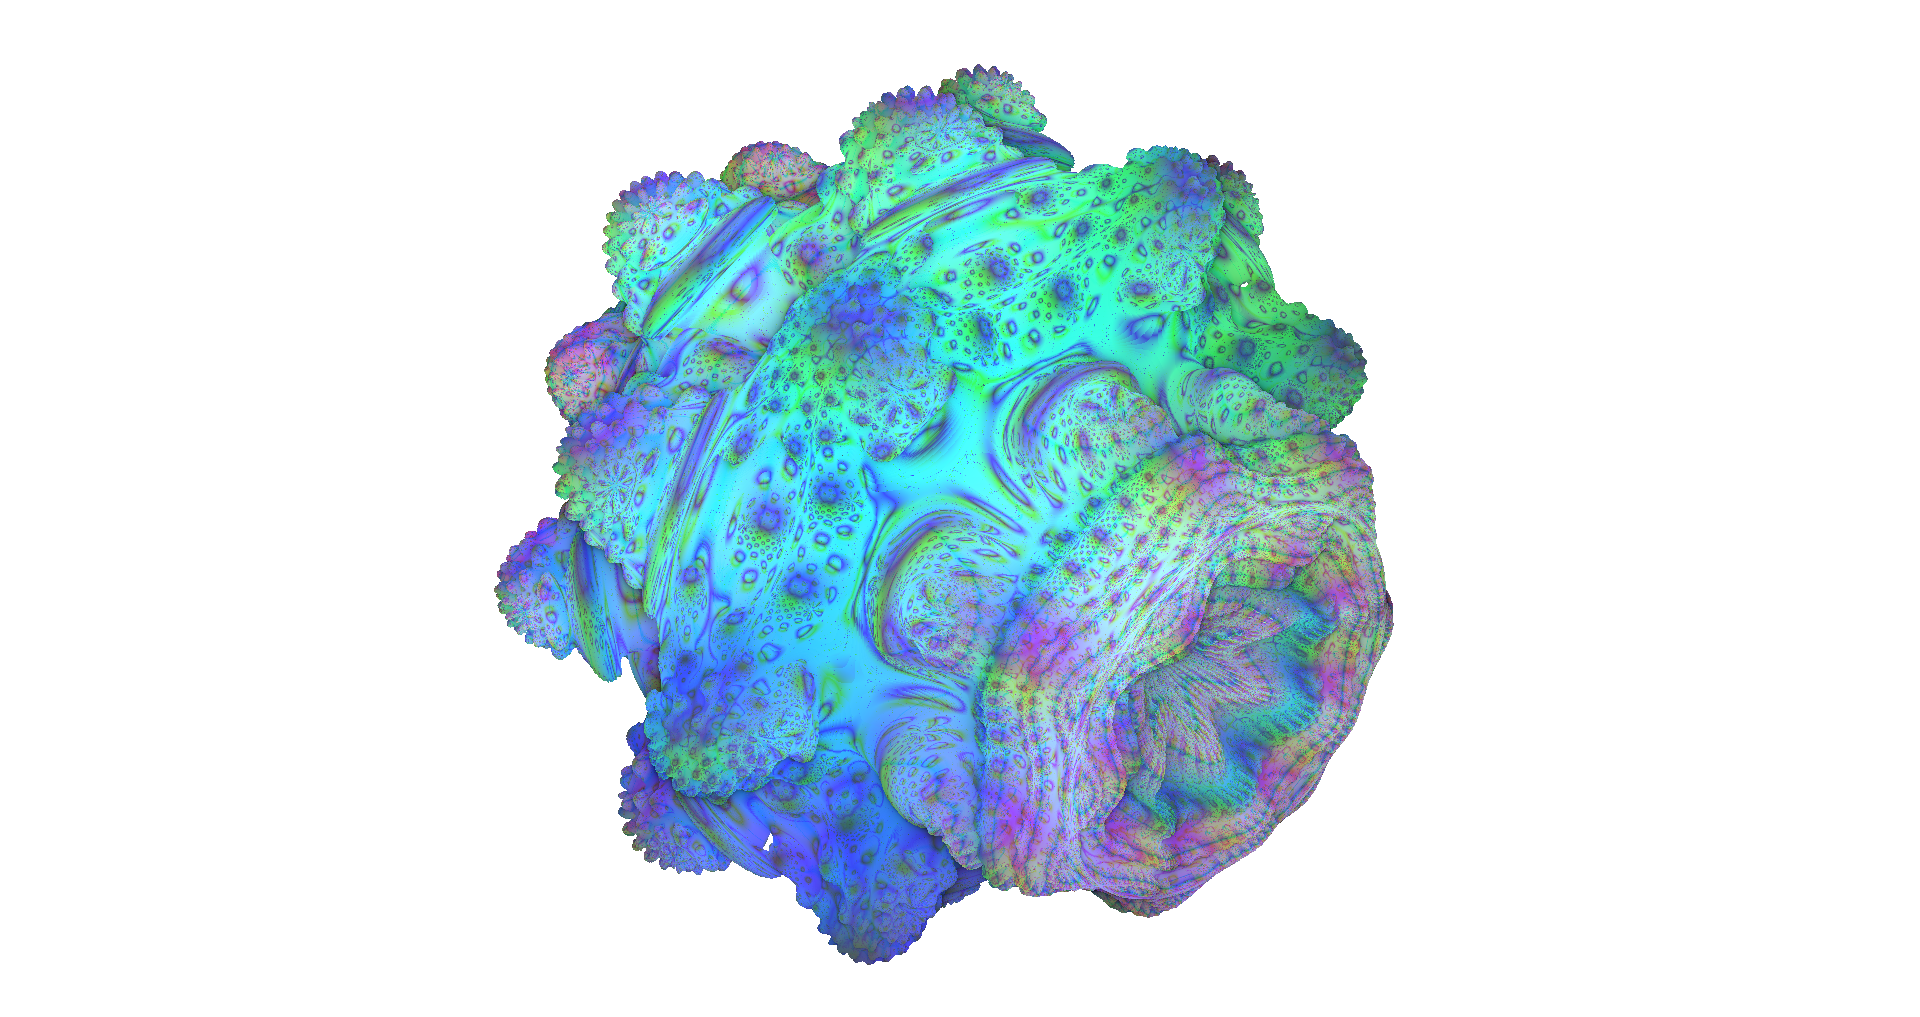
\includegraphics[width=\linewidth, frame]{Images/Results/Mandelbulb-View-01-Default}
		\caption{Mandelbulb: Default View.}
		\label{figure:mandelbulb-view-01-default}
	\end{subfigure}
	\hfill
	\begin{subfigure}[c]{0.45\linewidth}
		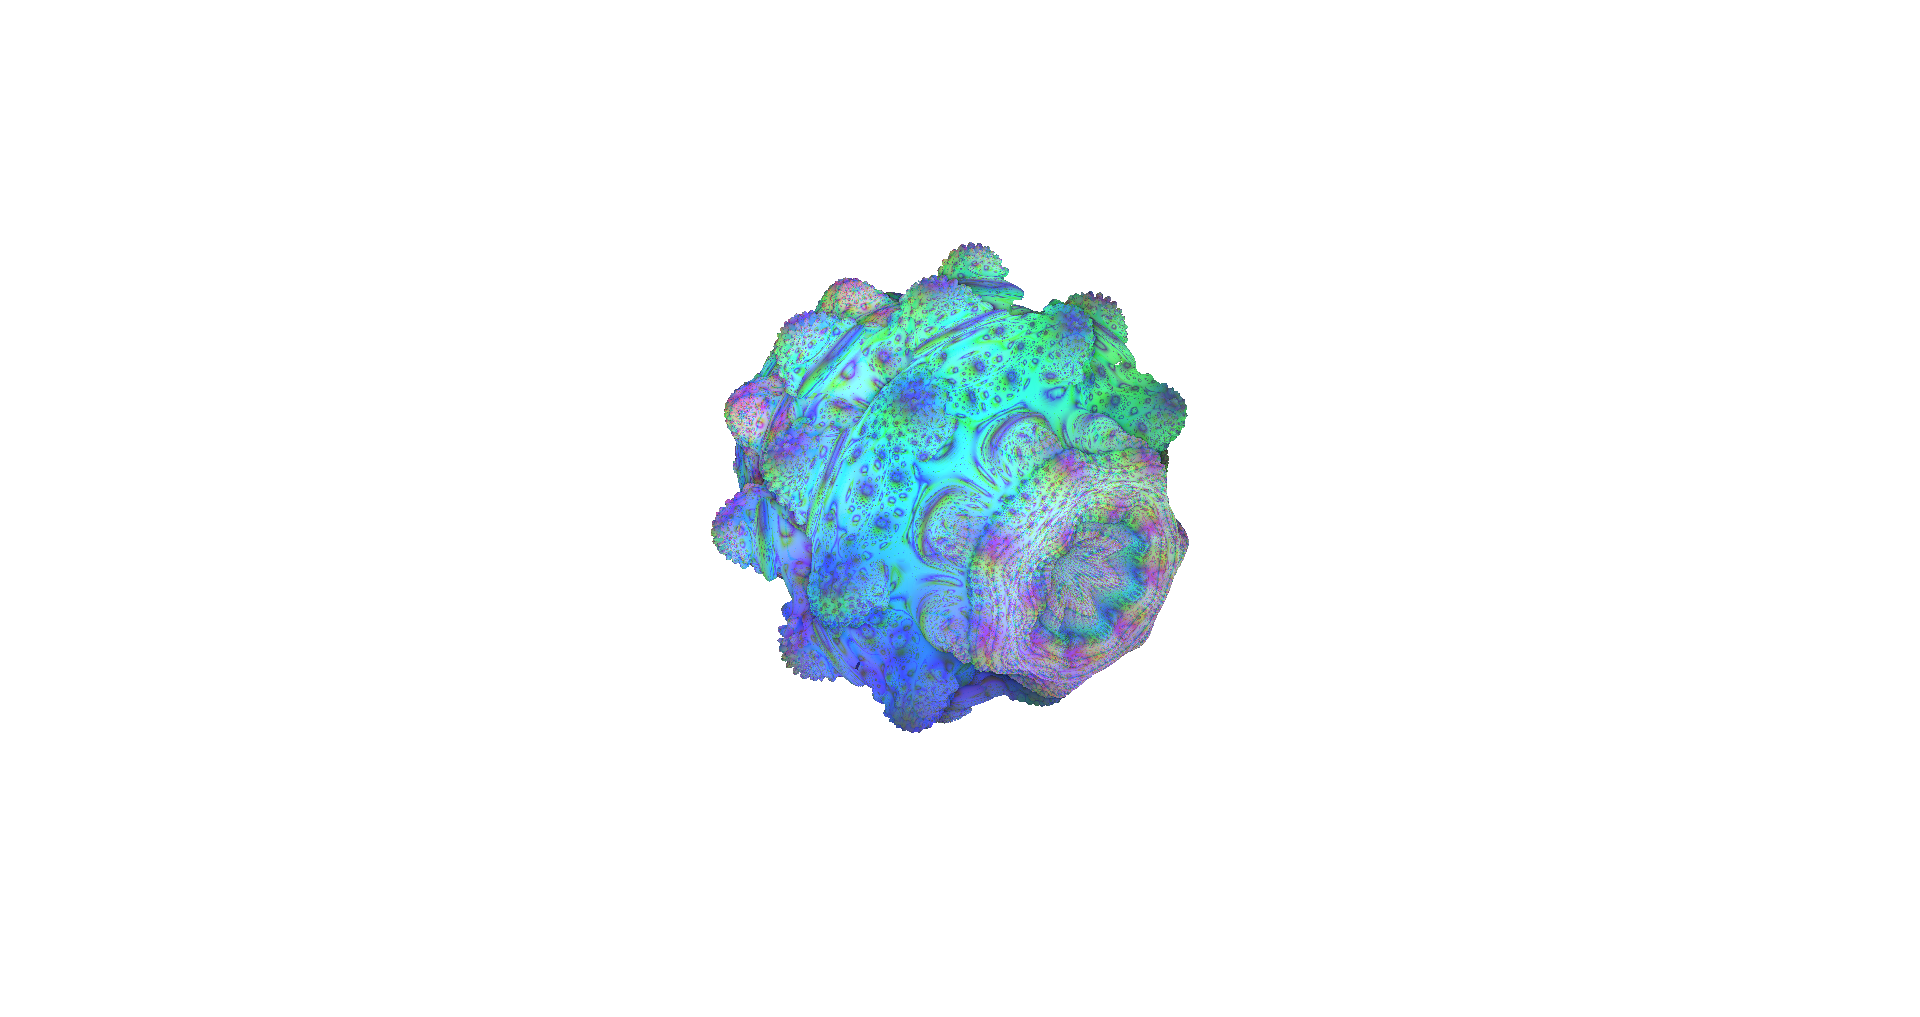
\includegraphics[width=\linewidth, frame]{Images/Results/Mandelbulb-View-02-Empty-Space}
		\caption{Mandelbulb: Zoomed Out View.}
		\label{figure:mandelbulb-view-02-empty-space}
	\end{subfigure}
	\hfill
	\begin{subfigure}[c]{0.45\linewidth}
		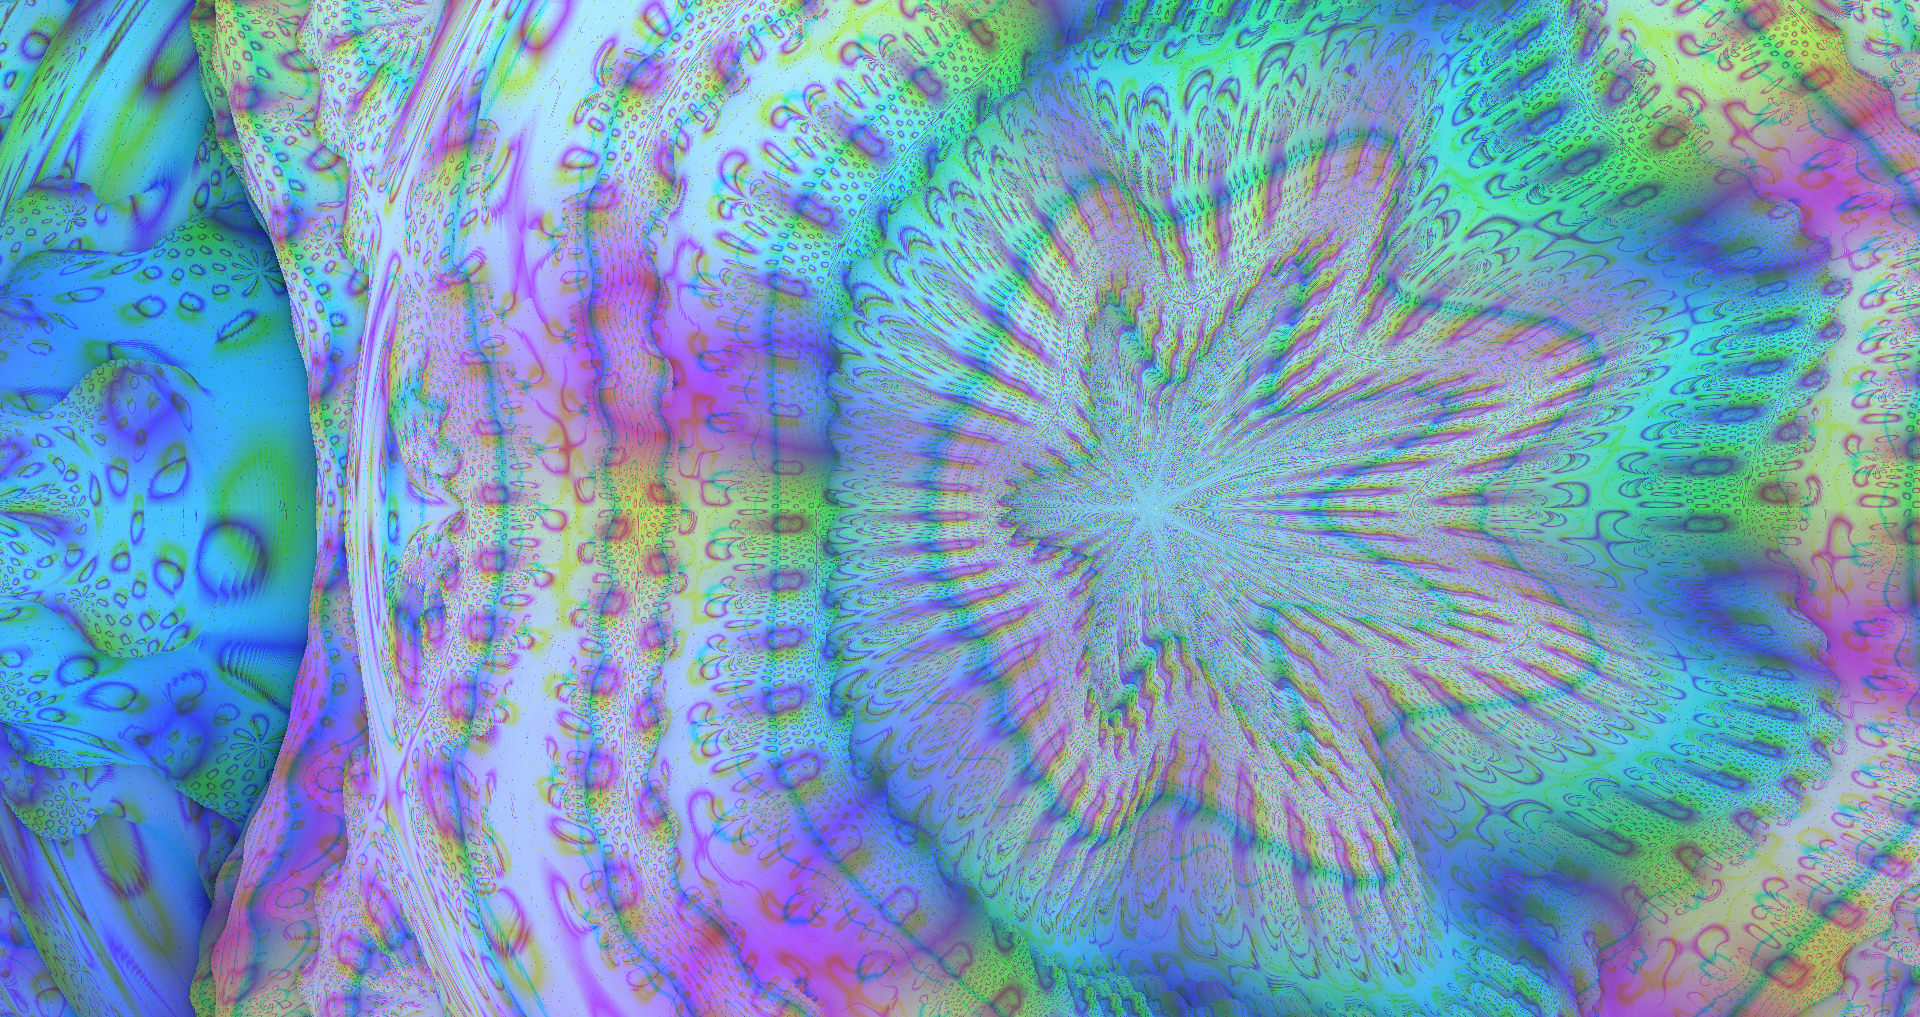
\includegraphics[width=\linewidth, frame]{Images/Results/Mandelbulb-View-03-No-Space}
		\caption{Mandelbulb: Zoomed In View.}
		\label{figure:mandelbulb-view-03-no-space}
	\end{subfigure}
	\hfill
	\begin{subfigure}[c]{0.45\linewidth}
		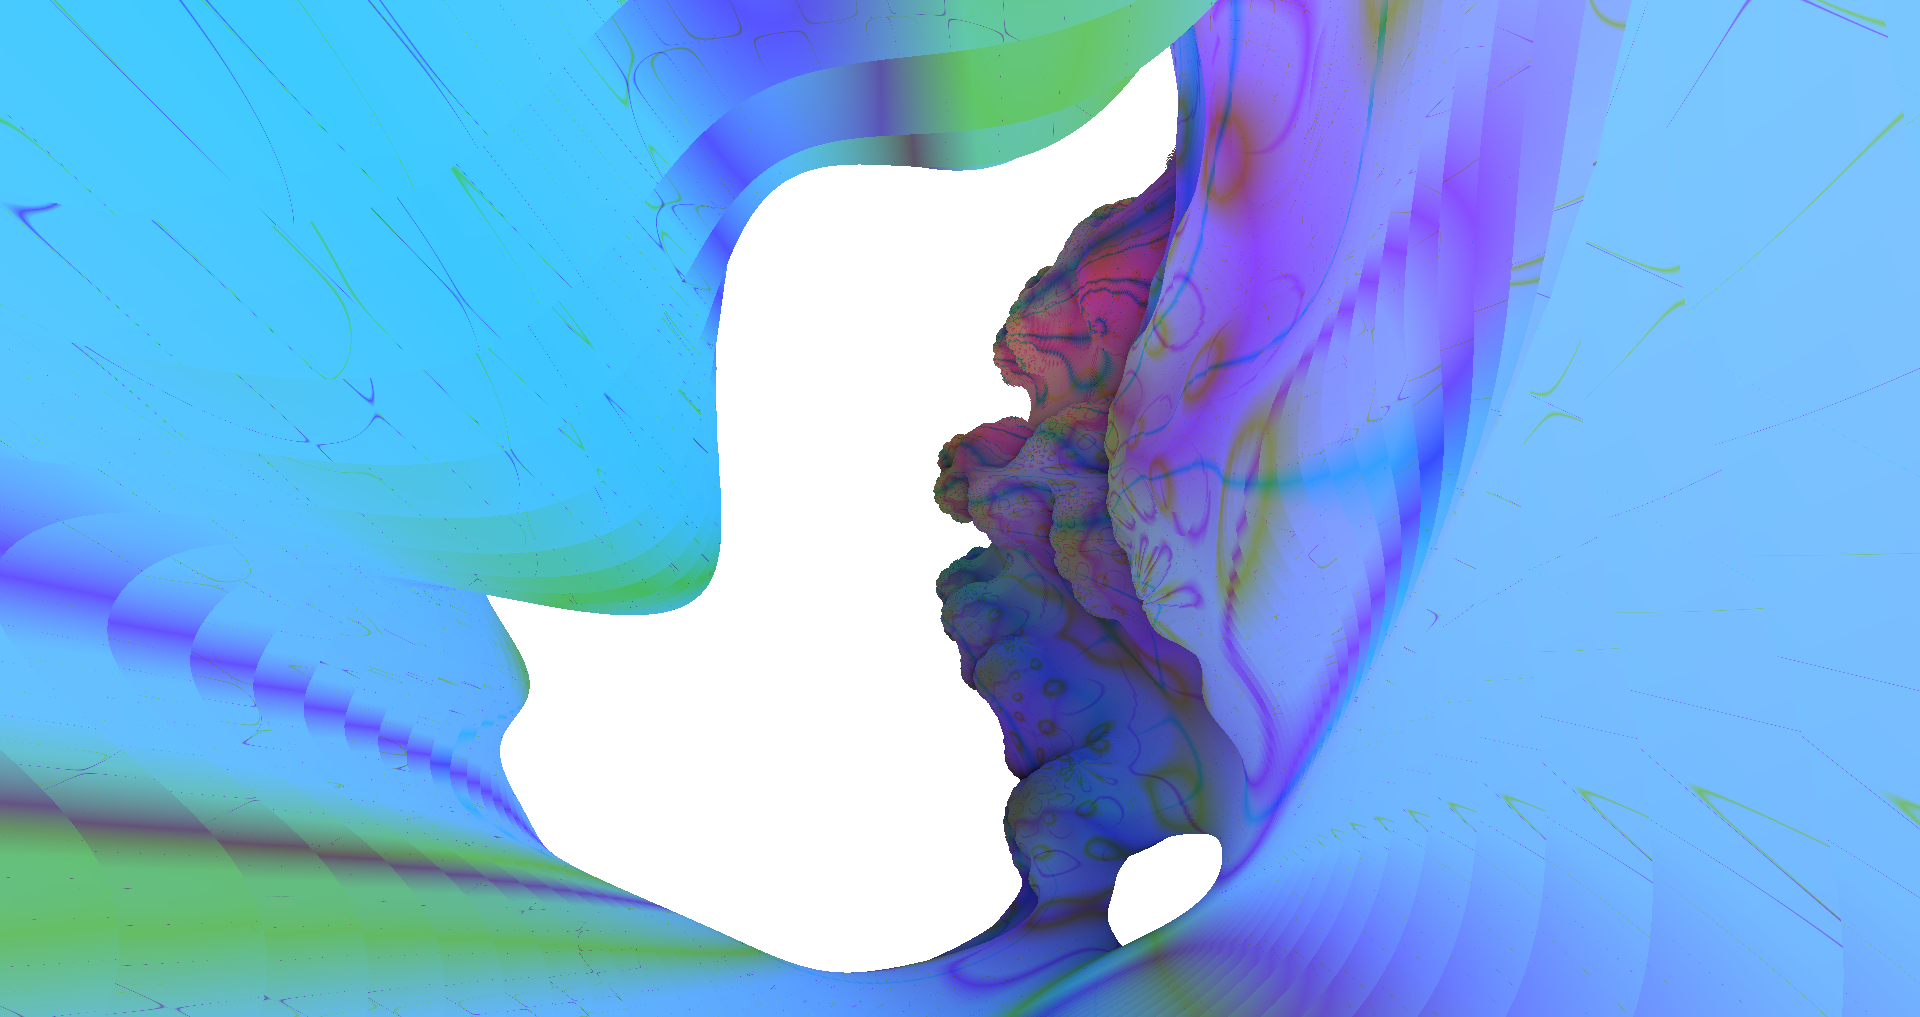
\includegraphics[width=\linewidth, frame]{Images/Results/Mandelbulb-View-04-Bottleneck}
		\caption{Mandelbulb: Bottleneck View.}
		\label{figure:mandelbulb-view-04-bottleneck}
	\end{subfigure}

	\caption{Four representative views of the Mandelbulb fractal, used in performance tests.}
	\label{figure:mandelbulb-views}
\end{figure}

Figure \ref{figure:mandelbulb-views} shows the four representative views used for performance measurements. Figure \ref{figure:mandelbulb-view-01-default} shows the default view, which is not expected to be particularly well suited to any performance measurement, to get a general-case overview of the performance differences between the methods used. Figure \ref{figure:mandelbulb-view-02-empty-space} is the view intended to include the most empty space (short of simply turning around and not looking at the fractal at all), and by contract figure \ref{figure:mandelbulb-view-03-no-space} is intended to include the least. Lastly, figure \ref{figure:mandelbulb-view-04-bottleneck} includes a mix of depth, smoothness and some bottlenecks.

\subsubsection{Results}

Table <ref> below shows the raw performance for these static images, using unoptimized rendering, the signed distance field and the temporal cache, as well as performance differences. Differences are measured in terms of the positive or negative performance difference, in percent, achieved by each optimization method.

\begin{tabular}{||p{0.2\linewidth}|p{0.3\linewidth}|p{0.225\linewidth}|p{0.225\linewidth}||}
	\hline
	View & Unoptimized Time (ns) & SDF Time (ns) & SDF Difference (\%)\\
	\hline\hline
	Default & 0 & 0 & 0\\
	\hline
	Zoomed Out & 0 & 0 & 0\\
	\hline
	Zoomed In & 0 & 0 & 0\\
	\hline
	Bottleneck & 0 & 0 & 0\\
	\hline
\end{tabular}

\subsection{Temporal Caching Exclusive}

\section{Hall of Pillars Tests}

This fractal contains many bottlenecks (the ray has to pass close to lots of geometry before reaching any surface), so the temporal caching method is expected to perform better here than with the Mandelbulb, in terms of performance difference. A view with very simple geometry was also chosen because of this, as the prediction is that the temporal caching method will provide minimal benefit where these bottlenecks don't exist, the surface is very smooth, or the distance to the surface is very small.\newline

The signed distance field was very tricky to test, since the fractal does not fit neatly into a small box, like the Mandelbulb. Because of this, during tests for the signed distance field, a ray culling step was added. Any ray not destined to intersect with the main signed distance field area is not followed. This gives a sort of cross-section of the fractal, and this was what was used. This step was added to all tests to be compared with the test for the signed distance field, for consistency. The signed distance field is not expected to give a huge benefit here, as the relative expense of the distance estimator is not very high.

\subsection{View:}

\subsection{Temporal Caching Exclusive}